\chapter{Background}
\label{ch:background}

In this chapter the theoretical foundations for the succeeding work are treated. Firstly, the Medium Access Control (MAC) layer is introduced in the context of the OSI reference model. Successively, a glance on a number of different MAC protocols and mechanisms is taken, while discussing performance with respect to the challenges and goals in wireless transmission. The chapter concludes with describing the advantages of software-defined radio (SDR) and how GNU (GNU is not Unix) Radio can be used to support SDR.

\section{MAC Protocols}

\subsection{MAC Layer in the OSI Model}

The OSI (Open Systems Interconnection) model is a layered architecture that divides a telecommunication system into several manageable layers. It features seven layers, where the second layer - the Data Link Layer (DLL) - can be split into two sublayers. The focus of this thesis lies on the lower sublayer, which is MAC. The upper sublayer is Logical Link Control (LLC). Table \ref{tab:osi-layers} gives a short overview of the layers' responsibilities. We will now take a closer look at the MAC functionalities in IEEE 802.11 (WLAN) networks. 

\paragraph{MAC Functionalities} The MAC layer provides the functionalities to enable connection-less (datagram style) transfer of data between nodes. It transparently carries the data of the next higher - the LLC layer - as service data unit (SDU). Other important functions include frame delimiting and recognition, addressing of destination stations, conveying the source-address, protection against errors with frame check sequences and controlling the access to physical medium \cite{802-std}. In this thesis we will only examine physical medium access aspects. 

\begin{table}[b]
	\begin{center}
		\begin{tabular}{p{1cm}p{4cm}p{8cm}}
			\toprule
				Level & Layer & Principal Functionalities \\
			\midrule
				1 & Physical Layer & dealing with mechanical, electrical and timing interfaces of data transmission  \\
				2 & DLL: MAC Sublayer & controlling medium access and frame synchronization \\
				2 & DLL: LLC Sublayer & multiplexing to enable different network protocols coexist, flow control and error control \\
				3 & Network Layer & routing and congestion control \\
				4 &Transport Layer & transmission reliability, same-order-delivery, congestion avoidance  \\
				5 & Session Layer & token management, dialog control, synchronization \\
				6 & Presentation Layer & abstracting syntax and semantics of transmission, encryption \\
				7 & Application Layer & user application protocols, such as http, ftp, smtp and many more \\
			\bottomrule
		\end{tabular}\caption{Layers in the OSI model \cite{osi}} \label{tab:osi-layers}
	\end{center}
\end{table}

\subsection{Challenges for Wireless MAC Protocols}

Wireless MAC protocols have to tackle a few problems that do not occur in wired data exchange. Among them are the hidden node and the exposed node problem, which will be discussed by reference to Figure \ref{fig:hidden_exposed_node_problem}. Further challenges, such as energy limitations will also be delineated.

\subsubsection{The Hidden Node and the Exposed Node Problem}

\begin{figure}[tb]
	\label{fig:hidden_exposed_node_problem}
	\begin{center}
		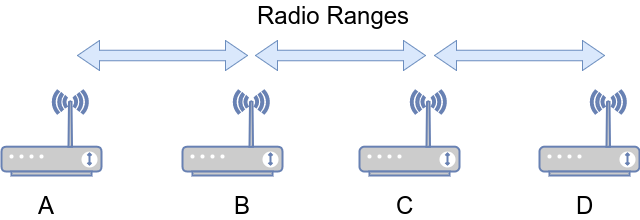
\includegraphics[width=12cm]{pictures/hidden_exposed_node_problem}
	\end{center}
	\caption{Setup to explain the hidden and exposed node problem. Each node can only reach its direct neighbors.}
\end{figure}

Suppose that the radio range of the nodes in \ref{fig:hidden_exposed_node_problem} is limited to the neighboring nodes and $A$ would like to transmit to $B$. If $C$ just started transmitting $A$ does not hear $C$ and falsely assume that the channel is idle and start transmitting, which leads to a collision. This is the hidden node problem \cite{Tanenbaum02}\cite{Gast05}.

For the same configuration, in another scenario $B$ would like to send to $A$ and $C$ is already transmitting to $D$. $B$ refrains from sending although collisions would only take place between $B$ and $C$, where it does not matter as both $B$ and $C$ are transmitters. This is the exposed node problem \cite{Tanenbaum02}\cite{Gast05} . 

\subsubsection{Power Problems}

% Citation needed for verification
Further challenges when designing MAC protocols include the power conservation when faced with constrained power resources, as e.g. in wireless sensor networks (WSN) where devices rely on batteries for their power supply. Attempts to reduce energy consumption have been made in several specialized, duty-cycle based MAC protocols for WSN such as Sensor MAC, Timeout MAC and Berkeley MAC as in more detail shown in Section \ref{sec:duty-cycle-mac}.

As a consequence of the constrained energy resources, WSN are especially susceptible to denial of sleep attacks, a special form of denial of service (DoS) attack, drastically increasing energy consumption and thus reducing the system lifetime. It is due to this fact that security is paramount in biomedical or military fields of application \cite{raymond09}. 


\subsection{Classification of MAC Protocols}

\begin{figure}[tb] \label{fig:mac-classification}
	\begin{center}
		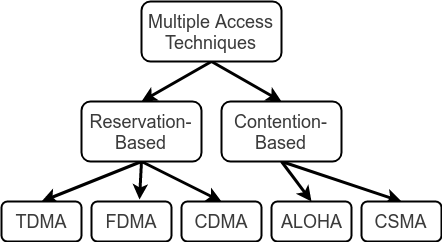
\includegraphics[width=0.5\textwidth]{pictures/mac_classification}
	\end{center}
	\caption{Classification of MAC techniques}
\end{figure}

Traditional MAC protocols can be classified into one of two groups: reservation-based and contention-based as depicted in Figure \ref{fig:mac-classification} \cite{Garg07}. The difference between them is that in reservation-based protocols a coordinator prevents collisions by assigning physical resources to devices, whereas in contention-based protocols no such infrastructure exists and nodes have to contend for channel utilization, hence the name. Another technique independent from these categories is to employ duty cycles (DC), where nodes continuously alternate between active and inactive periods. According to \cite{Bachir10} the appropriate choice of MAC protocol depends on a plethora of design-drivers such as requirements concerning throughput, latency, energy consumption and traffic patterns. 

We will proceed with discussing representative protocols of the two categories. Thereafter, we will take a look at a few protocols that use DC mechanism.

\subsection{Reservation-Based MAC Protocols}
\label{sec:reservation-mac}

Reservation-based protocols may implement an array of desirable features, but require knowledge of network topology in order to allow each node to communicate with every other on the basis of a centrally coordinated schedule. These features include reduced collisions, fairness among nodes or multiple transmissions at the same time. Owing to the fact that we do not incorporate reservation-based protocols in our experiments we will only briefly describe the basic principles of the time-division multiple access (TDMA), frequency-division multiple access (FDMA) and code-division multiple access (CDMA). 

TDMA is a representative protocol in this group, which divides time into slots. Each node is assigned to a unique slot during which it may transmit. As a result we obtain collision-free transmission, predictable scheduling delays, high throughput in heavy load situations and fairness among nodes. However, both the knowledge of topology and tight synchronization require large overheads or expensive hardware \cite{Bachir10}.

FDMA (FDMA) divides a frequency band into a number of channels. One or more may be assigned to each node. Receivers use bandpass filters to obtain the transmitted signal \cite{Garg07}.

CDMA is a digital spread-spectrum technique where multiple transmitters share the same frequency band and transmissions may occur at the same time. In this method transmitted signals are combined (XORed) with special \footnote{by special we mean that the signal has certain properties such as orthogonality and in some cases pseudo-randomness} sequences making the transmitted signal's frequency vary in order to avoid interference. The receiver has to follow along this variation of frequency (that is to say know the spreading code) when decoding to retrieve the original data signal, resulting in increasing security as a side effect \cite{Garg07}.

It is also possible to combine several of these techniques. Making use of this, the base station (eNB) of LTE in the licensed band coordinates traffic by assigning physical resource blocks (PRB) to devices. A PRB is a combination of a frequency and a time slot based on the reservation techniques of orthogonal FDMA (OFDMA) and TDMA. 

\subsection{Contention-Based MAC Protocols}
\subsubsection{ALOHA}
\label{sec:aloha}

ALOHA is arguably the most simple MAC protocol. Whenever a device wants to send data it just does so. The higher the channel load, i.e. transmissions per time unit, the more likely collisions will occur, which render all transmitted information useless.

The question is how likely it is that a collision does not occur. In other words, how efficient is an ALOHA channel? Making a statement requires a few preliminary assumptions as shown in \cite{Tanenbaum02}:

\smallskip

\begin{enumerate}
	\item We simplify the calculation by assuming a fixed frame length.
	\item The number of packets generated during a frame time is a Poisson-distributed random variable $X$.
	\item The channel load $G$ comprises of two portions: "new" and retransmitted frames.
\end{enumerate}

The probability mass function of the Poisson distribution and thus the probability of $k$ frames being generated during a given frame time amounts to:

\begin{equation}
	Pr(X=k) = \frac{G^k\cdot e^{-G}}{k!}
\end{equation}

The probability of zero frames being generated during the transmission of the frame is $Pr(X=0) = e^{-G}$ (assumption 3). If no collision occurs during the transmission of frame $F$, no other frame was sent during that transmission. Conversely, $F$ itself did not collide with a frame sent off prior to $F$. We conclude that the vulnerability period during which collisions may corrupt data is two frame times (assumption 2).

The probability that no frame other than the frame to be transmitted is generated during the two-frame-time vulnerability period is $P_0 = e^{-2G}$. The throughput $S$ is given by $S=GP_0 = Ge^{-2G}$.

The maximum throughput is achieved when $\frac{\partial S}{\partial G} \stackrel{!}{=} 0$:

\begin{eqnarray}
	& \frac{\partial S}{\partial G} & = \frac{\partial}{\partial G} Ge^{-2G} \\ 
	& & = e^{-2G}(1-2G) \\
	& & \stackrel{!}{=} 0 \\
	\Leftrightarrow & G & = 0.5
\end{eqnarray}
	
This means that for $G=0.5$ the throughput S reaches its maximum $S_\text{ALOHA,max} = \frac{1}{2e} \approx 0.18$. This result is very reasonable, since the transmission of a frame is vulnerable for the duration of two frame times, so the maximum is achieved when sending exactly every second slot, where a slot is equivalent to the frame time.

We note that, the throughput can be doubled with slotted ALOHA. In contrast to pure ALOHA, slotted ALOHA divides time into slots, where transmissions may only commence at the beginning of slots, which effectively halves the vulnerability period to only one slot, since frames transmitted prior to a frame $F$ cannot interfere with $F$ anymore. Thus, $S_\text{ALOHA,max} = \frac{1}{e} \approx 0.36$, reached at $G=1$. However, this comes at the cost of an additional frame delay of $t_\text{slot}$ in the worst case and $\frac{t_\text{slot}}{2}$ in the average case and the need for synchronization. 

As shown in Figure \ref{fig:aloha-csma-performance}, ALOHA's performance is discouraging and improvements over ALOHA were found. 

\subsubsection{CSMA}
\label{sec:csma}

\begin{figure}[tb]
	\label{fig:aloha-csma-performance}
	\begin{center}
		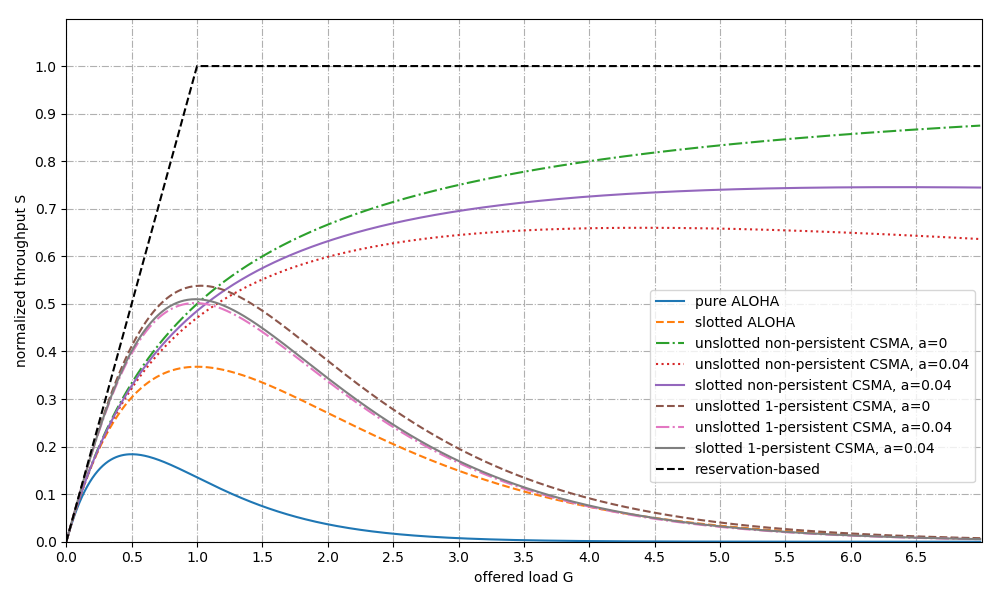
\includegraphics[width=\textwidth]{pictures/aloha_csma_performance}
	\end{center}
	\caption{Normalized throughput over offered load according to formulae in \cite{Tanenbaum02}, \cite{Garg07}, \cite{Bachir10},  , with $a=\tau/T_p$, where $\tau$ is the maximum propagation delay and $T_p$ the packet transmission time and under the assumptions made in Section \ref{sec:aloha}. }
\end{figure}

Main problem of ALOHA is the negligence of concurrent traffic in the channel. A solution to this problem is offered by "listen before talk" (LBT) mechanisms, which means in order to avoid collisions we make a clear channel assessment (CCA) and refrain from sending should it be busy. This is the simple, yet effective basic idea of carrier sensing multiple access (CSMA) which comes in three basic flavors, i.e. 1-persistent CSMA, non-persistent CSMA and p-persistent CSMA as depicted in Figure \ref{fig:csma-flavors} which will be discussed next.

\begin{figure}[tb] \label{fig:csma-flavors}
	\begin{center}
		\subfloat[1-persitent CSMA]{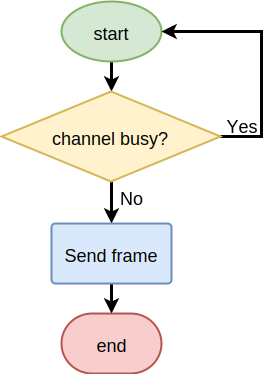
\includegraphics[width=0.22\textwidth]{pictures/csma_1_persistent}}
		\qquad
		\subfloat[non-persistent CSMA]{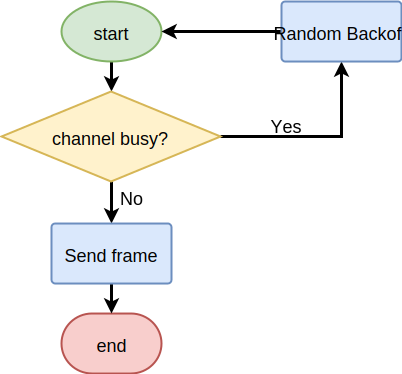
\includegraphics[width=0.31\textwidth]{pictures/csma_non_persistent}}
		\qquad
		\subfloat[p-persistent CSMA]{\includegraphics[width=0.35\textwidth]{pictures/csma_p_persistent}}
	\end{center}
\caption{The three basic flavors of CSMA}
\end{figure}

%LTE Unlicensed sends all control traffic through the licensed carriers, because in the unlicensed carrier the same quality of service, reliability and mobility cannot be achieved. The reason is that the unlicensed carrier is shared with multiple other systems that are out of the LTE operator's control. For this reason unlicensed carriers are only allocated for supplemental downlink (SDL) traffic.

\paragraph{1-Persistent CSMA}
\label{sec:csma-1-persistent}

If the channel is busy, 1-persistent CSMA waits until the channel becomes idle. As soon as the channel is found idle a frame is transmitted with a probability of 1, hence 1-persistent CSMA. If the frame collides with another, the node waits for a random backoff time and then the whole process is started all over again.

Despite being a substantial improvement over ALOHA, this protocol has at least two problems \cite{Tanenbaum02}:

\begin{itemize}
	\item Provided propagation delay is zero or negligible, collisions can still occur.  Imagine a three-node-scenario with nodes $A$, $B$ and $C$. $A$ is transmitting, while $B$ and $C$ are waiting for their turn. Once $A$ finished transmission $B$ and $C$ will simultaneously start their transmissions leading to collision.
	
	\item If propagation delay is not negligible the protocol suffers from an additional problem. In another scenario $A$ has just begun sending. $B$ will assume the channel is idle and send off his frame, since, due to the propagation delay, $B$ has not yet heard of $A$. This is why propagation delay may significantly hamper the performance of this protocol.
\end{itemize}  

\paragraph{Non-Persistent CSMA}

In order to alleviate 1-persistent CSMA's problem with several nodes trying to seize the channel as soon as it becomes idle, a less greedy attempt is made with non-persistent CSMA. Instead of continuously sensing the channel until it becomes idle, the nodes wait a random backoff time until they listen again. As a result, this protocol leads to better channel utilization with the downside of higher delays.

\paragraph{P-Persistent CSMA}

P-persitent CSMA is a protocol for slotted channels. Whenever a node $A$ wishes to send a packet, the channel is sensed. If the channel is found idle the node transmits its packet with a probability of $p$. With a probability $1-p$ the node defers its transmission to the next slot. This process is repeated until either the packet is sent or the channel is found busy again. In the latter case $A$ acts as though a collision had taken place and waits a random time until starting again \cite{Tanenbaum02}.

This flavor of CSMA can be regarded as a compromise between 1-persistent CSMA and non-persistent CSMA, where the choice of $p$ determines the greediness. The smaller $p$, the less greedy and thus the closer p-persistent CSMA approximates non-persistent behavior. An appropriate choice of $p$ can get the best out of both mechanisms: minimal delays as in 1-persistent CSMA, as well as high channel efficiency as in non-persistent CSMA.

\subsubsection{CSMA with Collision Detection}

A way to further improve the CSMA protocols is to immediately cancel transmissions once a collision is detected. There is no point in continuing these transmissions, as the transmitted data is lost in any case and aborting the transmission saves bandwidth, time and energy. 

CSMA with Collision Detection (CSMA/CD) is used on wired LANs and serves as basis of the wide-spread Ethernet. However, this mechanism is not extensively made use of in wireless networks. Concerning the reason, it is cardinal to understand that collision detection is an analog process. A collision is detected by comparing the received and transmitted energy or pulse width of the signal, which premises transmission and reception taking place simultaneously. This condition is seldom met for wireless nodes, which are mostly half-duplex. The reason for this lies in the conservation of energy, since wireless signals spread in all directions around their origin and thus degrade exponentially with the distance. Furthermore, wireless channels are typically much more noisy than their wired counterparts and suffer from multipath fading. To make up for the loss in signal strength we would have to employ expensive signal processing in order to recover fainter signals. Alternatively, we could increase the transmit power, but this increases interference with other nodes, as well as energy consumption.

\subsubsection{CSMA with Collision Avoidance}
\label{sec:csma-ca}

\begin{figure}[tb]
	\label{fig:virtual_carrier_sensing}
	\begin{center}
		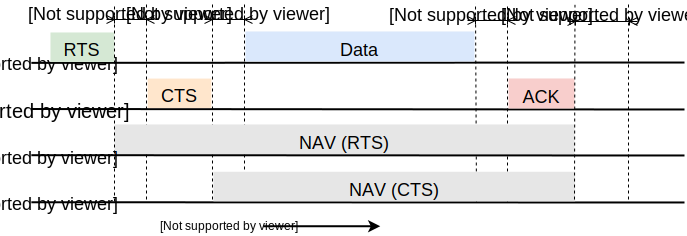
\includegraphics[width=14cm]{pictures/virtual_carrier_sensing}
	\end{center}
	\caption{Virtual carrier sensing in CSMA/CA, as described in \cite{Tanenbaum02} and \cite{Gast05}}
\end{figure}

IEEE 802.11 is a set of physical layer (PHY) and MAC specifications for wireless local area networks (WLANs). When the dominant mode of operation, the so-called distributed coordination function (DCF) is employed CSMA/CA is used in the MAC layer, which we will discuss next in accordance to \cite{Gast05} and \cite{Garg07}. 

As depicted in Figure \ref{fig:virtual_carrier_sensing} there are specific intervals of given length between each of the frames. Varying lengths of these interval types serve the purpose of prioritizing certain frames over others.

The short interframe spacing (SIFS) is the interval until the next control frame or next fragment (of a fragmented data frame) may be sent. SIFS is designed to allow one node out of the two nodes in dialog to have a higher priority to access the channel than uninvolved nodes. The longer interval DCF interframe spacing (DIFS) is the interval after which any station may try to seize the channel for their transmission.

For the sake of completeness, we briefly mention two further intervals used in IEEE 802.11, namely point coordination function interframe spacing (PIFS) and extended interframe spacing (EIFS). If IEEE 802.11 is operates in an alternative mode of operation, where a node acts as point coordinator of traffic the standard prescribes an interval of length PIFS to allow the controlling node to send certain control (beacon and poll) frames. EIFS is used to report the reception of a bad or unknown frame and due to the low priority of this action is the longest interval among the mentioned four. 

Physical carrier sensing takes place in these intervals. If a node wants to transmit a packet and the channel is sensed busy in one of these intervals then the node defers its transmission and launches the binary exponential backoff (BEB) procedure \cite{Gast05}. With BEB a node picks a slot in the so-called contention window (CW). The picked slot is just a random integer and the contention window is a range lower-bounded by zero and upper-bounded by $2^{n+m}-1$, where $m$ is a fixed integer, $2^m$ called minimum CW ($CW_\text{min}$) and $n=0$ for the moment. After picking the slot the node waits for $t_w = \text{\#slot} \cdot t_s$, where $\text{\#slot}$ is the number of the slot, $t_s$ a constant called backoff slot duration or simply backoff slot. After $t_w$ has elapsed the channel is sensed again. In the case it is sensed busy again the whole BEB procedure is repeated with $n$ incremented by 1, thus the CW doubled, hence \textbf{binary exponential} backoff.  The motivation for $CW_\text{min}$ is to greatly reduce the chance that two contending nodes pick the same slot in the first round of BEB defeating the purpose of BEB. The BEB mechanism is also used if collisions occur. Once a data frame is transmitted a timer is started, which is canceled when the corresponding ACK is received. If the timer runs out, i.e. no ACK was received, a collision is assumed and a round of BEB precedes the next try.    

Beside physical carrier sensing, another mechanism, namely virtual carrier sensing using RTS/CTS exchange is optionally employed to mitigate the problems caused by hidden nodes. In order to explain these mechanisms we refer to the setup of Figure \ref{fig:hidden_exposed_node_problem}. Figure \ref{fig:virtual_carrier_sensing} visualizes the chain of events whose explanation follows.

$B$ wants to send to $C$, hence issues a request to send (RTS). Every node receiving the RTS remains silent, except for $C$ that in response to the RTS creates a clear to send (CTS) frame. Not only $B$ receives this CTS frame, but also $D$, a hidden node from $B$'s point of view. Upon reception of CTS $D$ is silenced as well. Therefore, RTS/CTS is addressing the hidden node problem. RTS/CTS are frames of 30 bytes length containing the length of the frame that, in this case, $B$ wants to transmit. Based on this length, $A$ and $D$ setup the so-called network allocation vector (NAV), which are node-internal timers reminding $A$ and $D$ that the channel is still in use. This mechanism is called virtual carrier sensing due to the fact that the nodes defer their transmission based on the information received through other frames.

\subsubsection{Licensed Assisted Access}
Generally\footnote{for both license assisted access (LAA) as well as LTE-U}, the unlicensed band is only used to enhance the downlink rate in LTE traffic. The procedure of allocating additional carriers is called carrier aggregation (CA), and due to its limitation to downlink traffic more specifically supplemental downlink (SDL) CA. All control traffic is still sent through the licensed bands as it may exclusively be used by the licensee and thus is generally more reliable in terms of quality of service \cite{qualcomm15}.
One principal approach to ensure harmonious coexistence of LTE and Wi-Fi in the unlicensed band is License Assisted Access (LAA), relying on LBT. Since the LBT mechanism of LAA largely resembles CSMA/CA\footnote{actually CSMA/CA hybrid coordination function (HCF) enhanced distributed channel access (EDCA), where data packets with higher priority have a higher chance of being sent.} it seems quite natural to assume it will coexist better with Wi-Fi \cite{kwon17}. The other one is LTE-U which uses DCs and is discussed in Section \ref{sec:lteu}. 

\subsection{Duty-Cycle MAC Protocols} \label{sec:duty-cycle-mac}  

In duty-cycle MAC schemes nodes repeatedly alternate between active and inactive phases. In some protocols, especially in those designed for WSNs, nodes may sleep when inactive to reduce idle listening and thus energy consumption. Due to increased contention during active phases these protocols are mostly designed for limited contention traffic situations as in WSNs. The fraction of an active period in a cycle is called duty factor.

\subsubsection{LTE-U}
\label{sec:lteu}
LTE-U uses Carrier Sense Adaptive Transmission (CSAT), which tries to avoid primary channels of Wi-Fi transmissions and other LTE-U operators. If that is not possible, duty-cycles are dynamically adapted depending on Wi-Fi medium utilization (MU). If MU is below a certain threshold the DC is increased. If it is between that threshold and a higher one, the DC is kept constant, otherwise it is decreased \cite{qualcomm15}.

\subsubsection{Sensor MAC (SMAC)}

In SMAC the active period is divided into to a synchronization and a data transmission phase. During sync phase nodes transmit SYNC packets. Nodes receiving SYNC packets adopt the schedule carried by the packet and broadcast into their neighborhood. Nodes that follow the same schedule form a virtual cluster. Borderline nodes between virtual clusters adopt multiple schedules and thus have an increased duty factor. During contention period SMAC features the RTS/CTS exchange and fragments data frames, which are transmitted in a burst to reduce collision likelihood. The duty factor per schedule is predetermined on the basis of expected load as the result of an optimization problem on the competing goals of reducing idle listening and contention. The higher the duty factor the more idle-listening and the less contention occurs \cite{Bachir10}\cite{Demirkol06}.

\subsubsection{Timeout MAC (TMAC)}

While TMAC shares the same principle of schedule establishment with SMAC nodes adaptively vary duty factors depending on expected traffic. Furthermore, TMAC shifts all communication to the beginning of the active period. This allows nodes to sleep earlier should no traffic be detected during a certain time period. In variable load situations TMAC saves as much as five times more energy compared to SMAC at the cost of increased latency \cite{Bachir10}. 

\subsubsection{Berekeley MAC (BMAC)}

Still, TMAC maintains common active phases at high energy expenses. BMAC drops the requirement of maintaining common active phases. Instead payload is preceded by extended preambles such that every receiver is able to reliably detect packets. This has the effect of shifting energy expenses from the receiving to the sending side, which saves energy in low load applications such as surveillance. In BMAC CCA is based on outlier detection, instead of thresholding like in CSMA further reducing energy use \cite{Polastre04}. 

\section{Software-Defined Radio}
 
\subsection{Purpose of Software-Defined Radio}

Traditional radio equipment is "hardware-defined", i.e. that the signal processing runs on a specialized electrical circuit. This has the potential advantages of efficient energy use and cheap production at the cost of limited flexibility in operation. 

In SDR signal processing components such as filters, amplifiers, modulators, detectors and many more are implemented in software and mostly run on general-purpose processors, sometimes in combination with digital speech processors (DSPs) and field programmable gate arrays (FPGAs).

While the limitations of hardware-defined radios are acceptable for a number of applications, such as e.g. self-made radio receivers as shown in Figure \ref{fig:radio-receiver-circuits}, it is very desirable to get rid of these limitations for rapid prototyping of new technologies including but not limited to cognitive radio, software-defined antennas and wireless mesh networks. In the case of this thesis SDR simplifies studying the influence of different MAC mechanisms.

\begin{figure}[tb]
	\label{fig:radio-receiver-circuits}
	\begin{center}
		\subfloat[FM Receiver \cite{fm-receiver}]{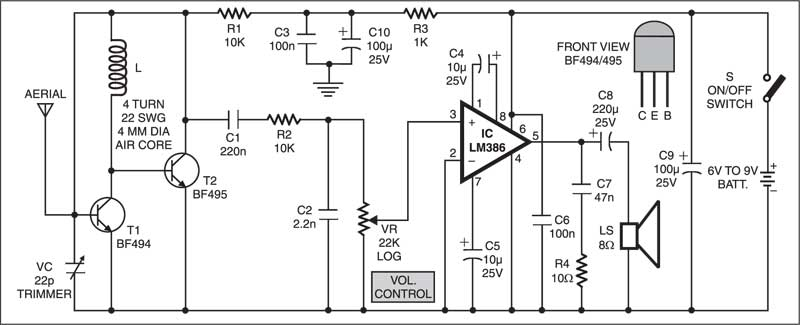
\includegraphics[width=0.5\textwidth,valign=c]{pictures/fm_radio_receiver_circuit}}
		\qquad
		\subfloat[AM Receiver \cite{am-receiver}]{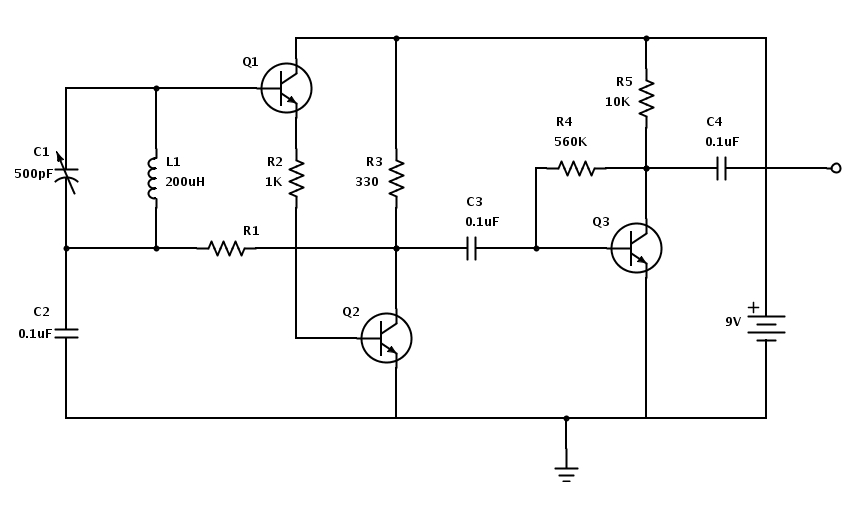
\includegraphics[width=0.4\textwidth,valign=c]{pictures/am_radio_receiver_circuit}}
	\end{center}
	\caption{Simple do-it-yourself (DIY) radio receiver circuit diagrams}
\end{figure}

\subsection{What is GNU Radio?}

\label{sec:gnu-radio}

The GNU Radio (GR) project is dedicated to the evolution of a free and open-source software development kit (SDK) enabling both the creation of actual software-defined radio, as well as simulated signal processing. Written in C++ and Python, GNU Radio also comes with the intuitive graphical software GNU Radio Companion (GRC) that allows creating block diagrams called flowgraphs simply by connecting signal processing blocks into a directed graph. Its target user market is not merely limited to research and industry, but also encompasses academia, government and private users \cite{gnuradio-about}.

A proprietary, well-documented alternative to GNU Radio is LabVIEW developed by National Instruments \cite{labview-about}. LabVIEW takes a purely graphical approach similar to GRC relying on block diagrams, but lacks the freedom of user-defined block creation with a programming language such as C++ or Python without extra efforts, such as buying a Python integration toolkit \cite{labview-python}.

Mathworks MATLAB/Simulink also provides a communication systems toolbox. However, the devices we used are not on the list of officially supported devices \cite{Matlab}.

\begin{figure}[t]
	\label{fig:gnuradio}
	% source: http://electronicsforu.com/electronics-projects/simple-fm-receiver 03.10.17
	% source: http://www.electroschematics.com/9043/am-receiver-circuit/ 03.10.17
	\begin{center}
		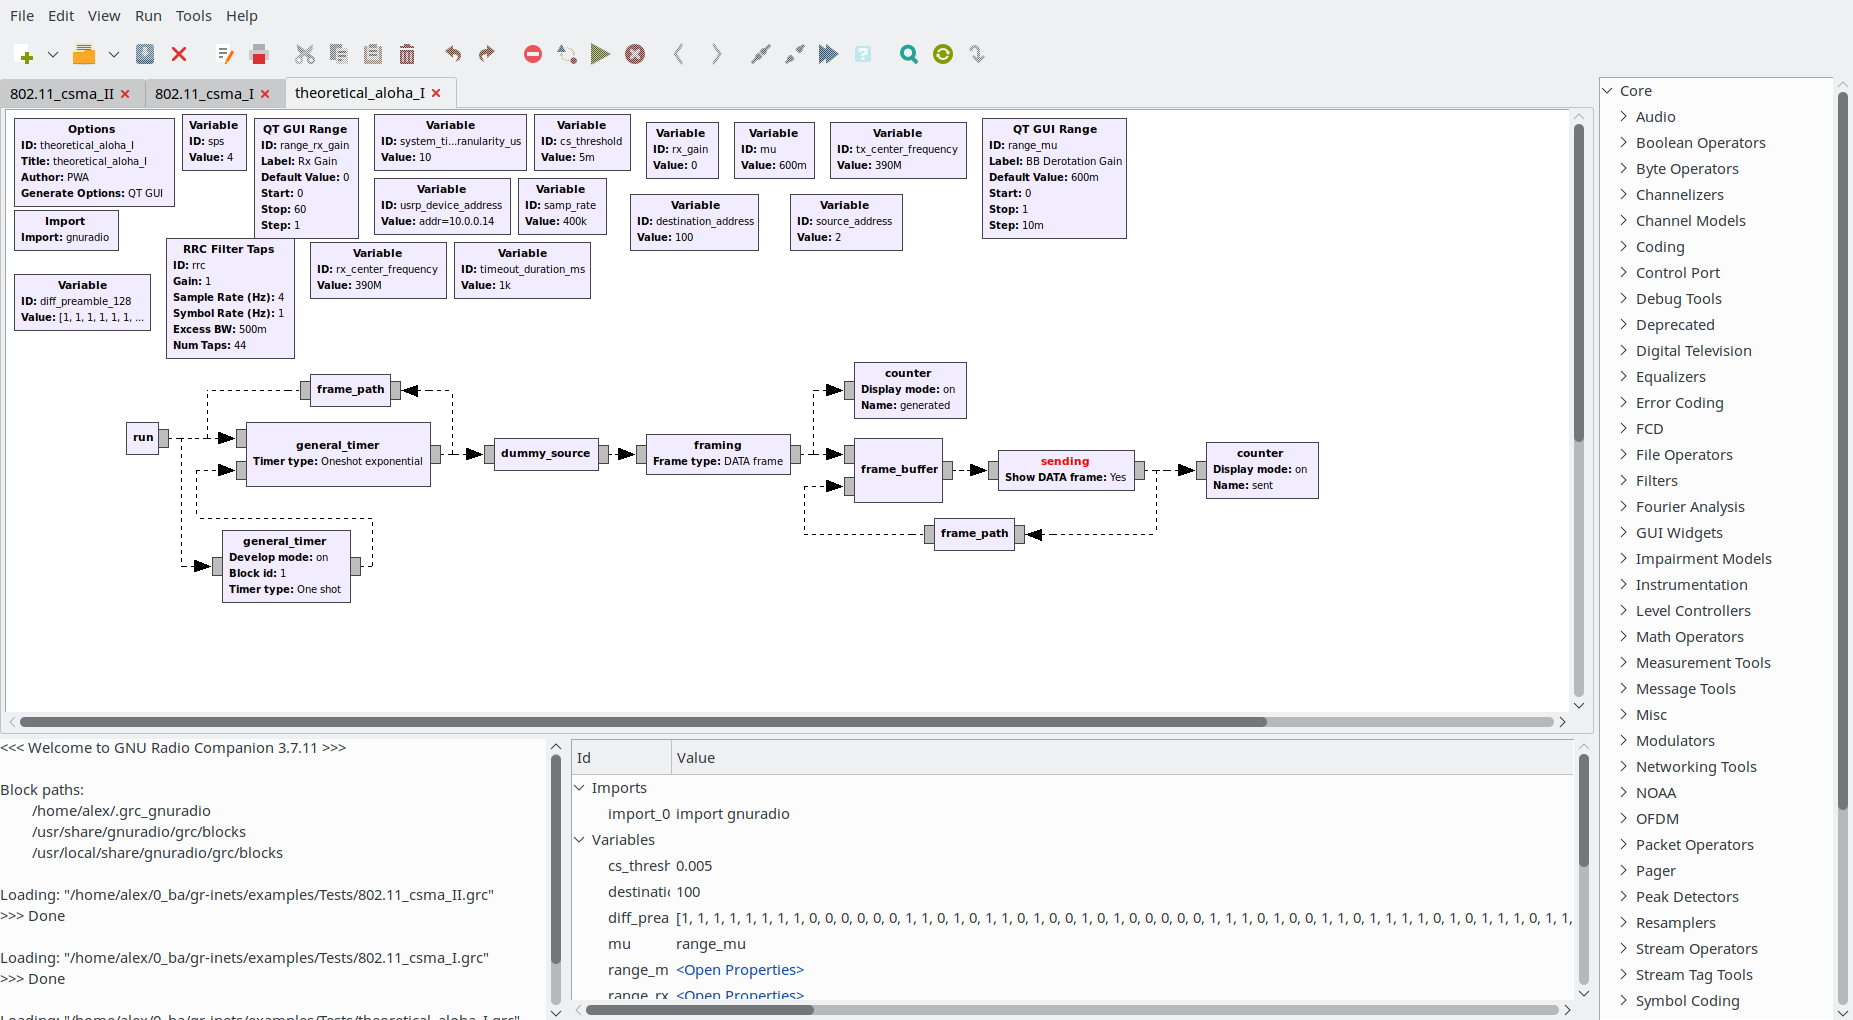
\includegraphics[width=0.9\textwidth,valign=c]{pictures/grc_ui}
	\end{center}
	\caption{GNU Radio Companion GUI}
\end{figure}

\subsection{Core Concepts of GNU Radio}

\subsubsection{Flowgraphs and Blocks}
\label{sec:flowgraphs}
The two most basic concepts of GNU Radio are flowgraphs and blocks. As mentioned in \ref{sec:gnu-radio} flowgraphs are directed graphs, whose nodes are functional blocks and whose vertices determine the direction of data flow \cite{GR1}. 

The behavior of these blocks is programmed in either Python or C++, where the latter is recommended for performance-critical applications, which is also why the blocks in our flowgraphs are all written in C++. If performance is less critical Python is a superior choice since it is more concise and allows faster prototyping as there is no need for compilation. Each block generally serves exactly one purpose for the sake of modularity. Blocks in turn can be composed of an arbitrary number of inner blocks, making extensive use of the modularity and hiding implementation complexity from the user, much like a blackbox in electrical circuits. These composed blocks are called hierarchical blocks. In our case the complete PHY layer is hidden in hierarchical blocks called "sending" and "receiving".

Blocks are connected through ports, which can either be input or output ports. Depending on which types of ports a block has, it can either be a source, sink or neither of the former. 
Each input port only consumes data of a specific data type. Similarly, each output port only produces data of a specific data type. The set of types ranges from integers, floating point and complex numbers to messages and a bunch of others. Since each block implements a certain function these ports can be regarded as input parameters and return values of a function, respectively.

\subsubsection{Message Passing and Stream Tags}

When designing packet-based protocols, such as MAC protocols it is of tremendous importance to be able to detect packet data unit (PDU) boundaries. For this purpose GR provides an asynchronous message passing system. A synchronous alternative is to attach so-called stream tags to the "infinite" stream of data. The former method is the right choice when designing MAC protocols due to the asynchronous nature of packet delivery \cite{GR1}\cite{GRDocs}.  

\subsubsection{Polymorphic Types and SWIG} 

Polymorphic types (PMT) are opaque data types that enable safe information exchange across blocks by serving as generic containers of data. Self-evidently, the original data type must be retained as a PMT class member. For thread-safety reasons PMT are immutable. We make extensive use of PMTs when passing messages. As an aside, note that the Python PMT class has some powerful tools unavailable its C++ counterpart, making use of Python's weak typing \cite{GRDocs}.

Simplified wrapper and interface generator (SWIG) is a software that helps to connect code written in C or C++ to a variety of scripting languages, such as in our case Python. This is achieved by generating a Python module from the C/C++ code with the help of an interface file. This "compatibility layer" is necessary, because blocks can be written in either Python or C++ as mentioned earlier.